%%%%%%%%%%%%%%%%%%%%%%%%%%%%%%%%%%%%%%%%%%%%%%%%%%%%%%%%%%%%%%%%%%
%%%%%%%% ICML 2010 EXAMPLE LATEX SUBMISSION FILE %%%%%%%%%%%%%%%%%
%%%%%%%%%%%%%%%%%%%%%%%%%%%%%%%%%%%%%%%%%%%%%%%%%%%%%%%%%%%%%%%%%%

% Use the following line _only_ if you're still using LaTeX 2.09.
%\documentstyle[icml2010,epsf,natbib]{article}
% If you rely on Latex2e packages, like most moden people use this:
\documentclass{article}

% For figures
\usepackage{graphicx} % more modern
%\usepackage{epsfig} % less modern
\usepackage{subfigure} 

% For citations
\usepackage{natbib}

% For algorithms
\usepackage{algorithm}
\usepackage{algorithmic}
\usepackage{amsmath}

% As of 2010, we use the hyperref package to produce hyperlinks in the
% resulting PDF.  If this breaks your system, please commend out the
% following usepackage line and replace \usepackage{icml2010} with
% \usepackage[nohyperref]{icml2010} above.
\usepackage[draft]{hyperref}

% Packages hyperref and algorithmic misbehave sometimes.  We can fix
% this with the following command.
\newcommand{\theHalgorithm}{\arabic{algorithm}}

% Employ the following version of the ``usepackage'' statement for
% submitting the draft version of the paper for review.  This will set
% the note in the first column to ``Under review.  Do not distribute.''
\usepackage{icml2010} 
% Employ this version of the ``usepackage'' statement after the paper has
% been accepted, when creating the final version.  This will set the
% note in the first column to ``Appearing in''
%\usepackage[accepted]{icml2010}


% The \icmltitle you define below is probably too long as a header.
% Therefore, a short form for the running title is supplied here:
\icmltitlerunning{CS 6784: Final report}



\begin{document} 

\twocolumn[
\icmltitle{Automated transcription of polyphonic piano music using structured SVM classification}

% It is OKAY to include author information, even for blind
% submissions: the style file will automatically remove it for you
% unless you've provided the [accepted] option to the icml2010
% package.
\icmlauthor{Charles Hermann}{cih5}
%\icmladdress{Your Fantastic Institute,
%            314159 Pi St., Palo Alto, CA 94306 USA}
\icmlauthor{Jonathan Shi}{js2845}
%\icmladdress{Their Fantastic Institute,
%            27182 Exp St., Toronto, ON M6H 2T1 CANADA}

% You may provide any keywords that you 
% find helpful for describing your paper; these are used to populate 
% the "keywords" metadata in the PDF but will not be shown in the document
\icmlkeywords{structral SVM, MIR, transcription, machine learning, polyphonic}

\vskip 0.3in
]

\begin{abstract} 
We investigate the use of maximum-margin CRF classifiers in the automated
transcription of polyphonic piano music.
Existing work on this problem has involved separate and independent smoothing
and classification steps. The use of a maximum-margin CRF classifier allows
us to unify these two steps. We present evaluation results against a
frame-by-frame one-vs-all SVM classifier.
\end{abstract} 


\section{Introduction}

\subsection{Motivation}
One of the major areas of research in music information retrieval (MIR) is
automated music transcription, the
process of creating a musical score from an audio recording. Though this
can be done manually by experienced musicians, this process is difficult
and time consuming. As a result, the ability to automatically transcribe
music has numerous positive ramifications in the musical community and the
MIR community. In addition, transcription presents an interesting and
difficult challenge even for seemingly easily versions of the task such as
transcribing piano solos. Several factors make this a difficult area of
study including but not limited to: the high-dimensionality of the
datasets, the large margin for error (both false positives and false
negatives), and the lack of a field-accepted feature vector/technique for
extracting the data. 

\subsection{Feature analysis}
An audio signal consists of a series of samples of wave displacement over time. See figure ~\ref{fig:wave} on page \pageref{fig:wave}.
As is often convenient, we process this audio input to obtain samples of
signal intensities in various frequencies over time.  This is called the
short-term fourier transform (STFT). See figure \ref{fig:freqs} on page \pageref{fig:freqs}.


Using the STFT, we obtain spectograms, which are plots of which
particular frequencies are present at any particular time within a signal. See figure \ref{fig:single_freqs} on page \pageref{fig:single_freqs}.

Features that we observe within a spectogram include:
\begin{description}
\item[Overtones.]
  Each note, when played, consists of a fundamental frequency, which is the
  pitch of the note that we perceive, as well as a set of overtones at
  integer multiples of the original frequency.
  % \cite{} TODO
\item[Partials.]
  A partial of a note is one of the theoretically pure sine wave constituents of
  that note. The fundamental frequency will be one of the partials, and each
  overtone will contribute another partial. Rather than being pure sine waves,
  which would show up in the spectograph as straight think horizontal lines, in
  reality each partial will be a bit fuzzy and show up as blurred horizontal
  bars in the spectograph.

  It is also notable that some partials might fade faster than others, for a
  particular note, and that they sometimes disappear entirely for brief moments
  before reappearing within the same note.
\item[Missing fundamentals.] 
  In certain cases, a human will hear a note being played at a certain pitch
  even if the fundamental frequency is omitted from the signal. This is because
  the human audio processing system can infer the fundamental frequency from
  the present overtones. 
  % \cite{} TODO
\item[Beat frequencies.]
  When two distinct frequencies are played over each other, they give rise to
  a beat frequency equal to the difference of the two original frequencies.
  Human ears hear these as subjective tones, and some previous attempts have
  incorrectly detected beat frequencies as new note onsets
  \cite{marolt2004connectionist}. 
\end{description}



Previous work on this task have focused mostly around:
\begin{enumerate}
\item Discriminative SVMs and CRFs trained to detect individual notes
  or note events at the time windows when they occur
  \cite{ryynanen2005polyphonic} \cite{poliner2006discriminative}
  \cite{gang2009polyphonic}.
\item Hidden Markov networks for particular chords \cite{raphael2002automatic}.
\item Neural network approaches using recurrent networks
  \cite{marolt2004connectionist} \cite{bock2012polyphonic}.
\item Estimation and then subtraction, or expectation-maximization, of sets of
  predetermined overtones corresponding to each possible fundamental frequency.
  \cite{5946322}.
\end{enumerate}

  Some previous work has incorporated feature sets from spectrograph
  data that have been specially tuned for the transcription task.
  These include a pitch salience function \cite{5946322}, deeply learned
  feature sets \cite{nam2011classification}, features acquired via sparse
  nonnegative matrix factorization \cite{costantini2013nmf}, and features
  generated by a model of human inner ear hair cells
  \cite{marolt2004connectionist}. Also feature sets have
been obtained via deep learning \cite{nam2011classification} and sparse
nonnegative matrix factorization \cite{costantini2013nmf}, which have performed
better in classification-based transcription than manually specified features.

Difficult points for previous classifiers have also included octave errors,
since notes that are an octave apart from each other are very similar in
their partials \cite{bock2012polyphonic} \cite{poliner2006discriminative}.
Previous methods also experienced
difficulties in distinguishing which notes were onset and which were just held
when some note onset event was detected \cite{marolt2004connectionist}.

There has been previous work \cite{gang2009polyphonic} dealing with the use
of max-margin methods to transcribe musical notes. Our approach differs
substantially from theirs because they apply a max-margin Markov network to
classify sets of pre-segmented partials according to which instrument they
belong to. Meanwhile we skip the analysis of partials and attempt to classify
notes directly from the spectograms as features. 


\section{Methods}
\newcommand{\x}{\mathbf{x}}
\newcommand{\y}{\mathbf{y}}
\newcommand{\w}{\mathbf{w}}
\newcommand{\f}{\mathbf{f}}

% TODO
The core method being introduced is to leverage a
maximum-margin Markov model \cite{Taskar03max-marginmarkov} for classification
on spectral data, which improves
upon an HMM by using SVM techniques to find optimal separating hyperplanes
that respect correlations between components of output labels.

%In addition, we expect the maximum-margin Markov framework introduced in
%\cite{anguelov2005discriminative} to be of use.
% TODO not sure if this is true?

\subsection{Notation}
Some notation to help in formalization:

We'll use $A \otimes B$ denotes the outer product of two vectors. More
explicitly:
\[ (A \otimes B)_{n_Bi+j} = A_iB_j, \]
where $n_B$ is the number of components in $B$. Informally, this is
a new vector representing the set of all pairwise products of components of
$A$ with components of $B$.

Similarly, $A \oplus B$ will denote the direct sum, so that:
\[ (A \oplus B)_i =
      \begin{cases} A_i & \text{ if $i \le n_A$} \\
                    B_{i-n_A} & \text{ if $i > n_A$}.
      \end{cases}
\]
Informally, this is simply concatenating the two vectors $A$ and $B$.

\subsection{Maximum-margin Markov network}
% TODO(FIX THE SECTION)
We set up a Markov network such that correlations exist only between:
\begin{enumerate}
\item different pitches within the same time window, and
\item pitches that occur in adjacent time windows.
\end{enumerate}
% TODO diagram of Markov network?

% TODO wait... this isn't even a Markov chain...

In the framework of Markov networks, we minimize
an energy function $\psi(\x,\y)$, which we will decompose as
$\psi(\x,\y) = \sum_t \psi_t(\x,\y)$, with one energy function per time window
in the signal. A maximum-margin Markov network then sets:
\[ \psi_t(\x,\y) = \exp[\w^T\f_t(\x,\y)], \]
for some vector $\w$ that we train using SVM methods, and some vector of
features $\f_t(\x,\y)$.

\subsection{Features}\label{features}
We use the features suggested in \cite{poliner2006discriminative}.
We use as our features essentially raw spectral data:
A STFT of the audio data sampled at 5.5 kHz,
an 1024-point Hanning window (185 milliseconds),
and an 80-point advance between adjacent windows
(for a 14.5-millisecond hop between successive frames).

Since we are training a model that leverages correlations in note labels
between adjacent time points, we also include the features from adjacent
time points. This way the Markov network can leverage \emph{changes} in
intensity at each frequency in order to help predict changes in note labels.

Thus, if we let $\x_{\omega}(t)$ denote the signal intensity at frequency
$\omega$ and time $t$, and similarly let $\y_{\rho}(t)$ denote an indicator
variable for whether pitch $\rho$ is on at time $t$, our expression for the
feature vector is:
\begin{align*}
  \f_t(\x,\y) &= h_t(\y) \oplus
      \\& [\x(t+1) \oplus \x(t) \oplus \x(t-1)]
      \\&\otimes [\y(t+1) \oplus \y(t) \oplus \y(t-1)],
\end{align*}
where $h_t$ encodes the Markov transition probabilities for each particular
time step of the note labeling.

\section{Data}
Training and testing data were sourced from the MAPS dataset 
\cite{emiya2010multipitch}, a set of 31 GB of piano recordings in .wav format,
recorded on varying pianos and in varying acoustic environments, with ground
truth transcription labels provided.

We downsampled the original 44.1kHz recordings by a factor of 8 to
obtain 5.5kHz signals. After extracting the windows as described in section
\ref{features}, we then used the first 2000 windows (or 30 seconds) of each
recording.

We separate our data into training and test sets.% TODO

\section{Evaluation}
% TODO
We evaluate according to the standard set in \cite{poliner2006discriminative} and \cite{bock2012polyphonic}.
In both of these papers, they worked with a large library of wav files accompanied by midi files. Their software produced
output which could be directly compared with the midi files and measured for: notes correctly predicted, notes failed to be predicted, and notes incorrectly predicted.

We first constructed and tested the method used by \cite{poliner2006discriminative} in identifying individual notes. In an attempt to replicate Figure 2, we tested the classification accuracy of an SVM trained to recognize middle C (M60). For this, we used the ISOL directory (individual notes, chromatics, trills, repeated notes, stacatto) as the training data and the RAND directory (random chords) as the test data. Despite following the method and features described in \cite{poliner2006discriminative} we found that the baseline accuracy of the SVM did not change as the number of samples increased significantly.

\begin{figure}
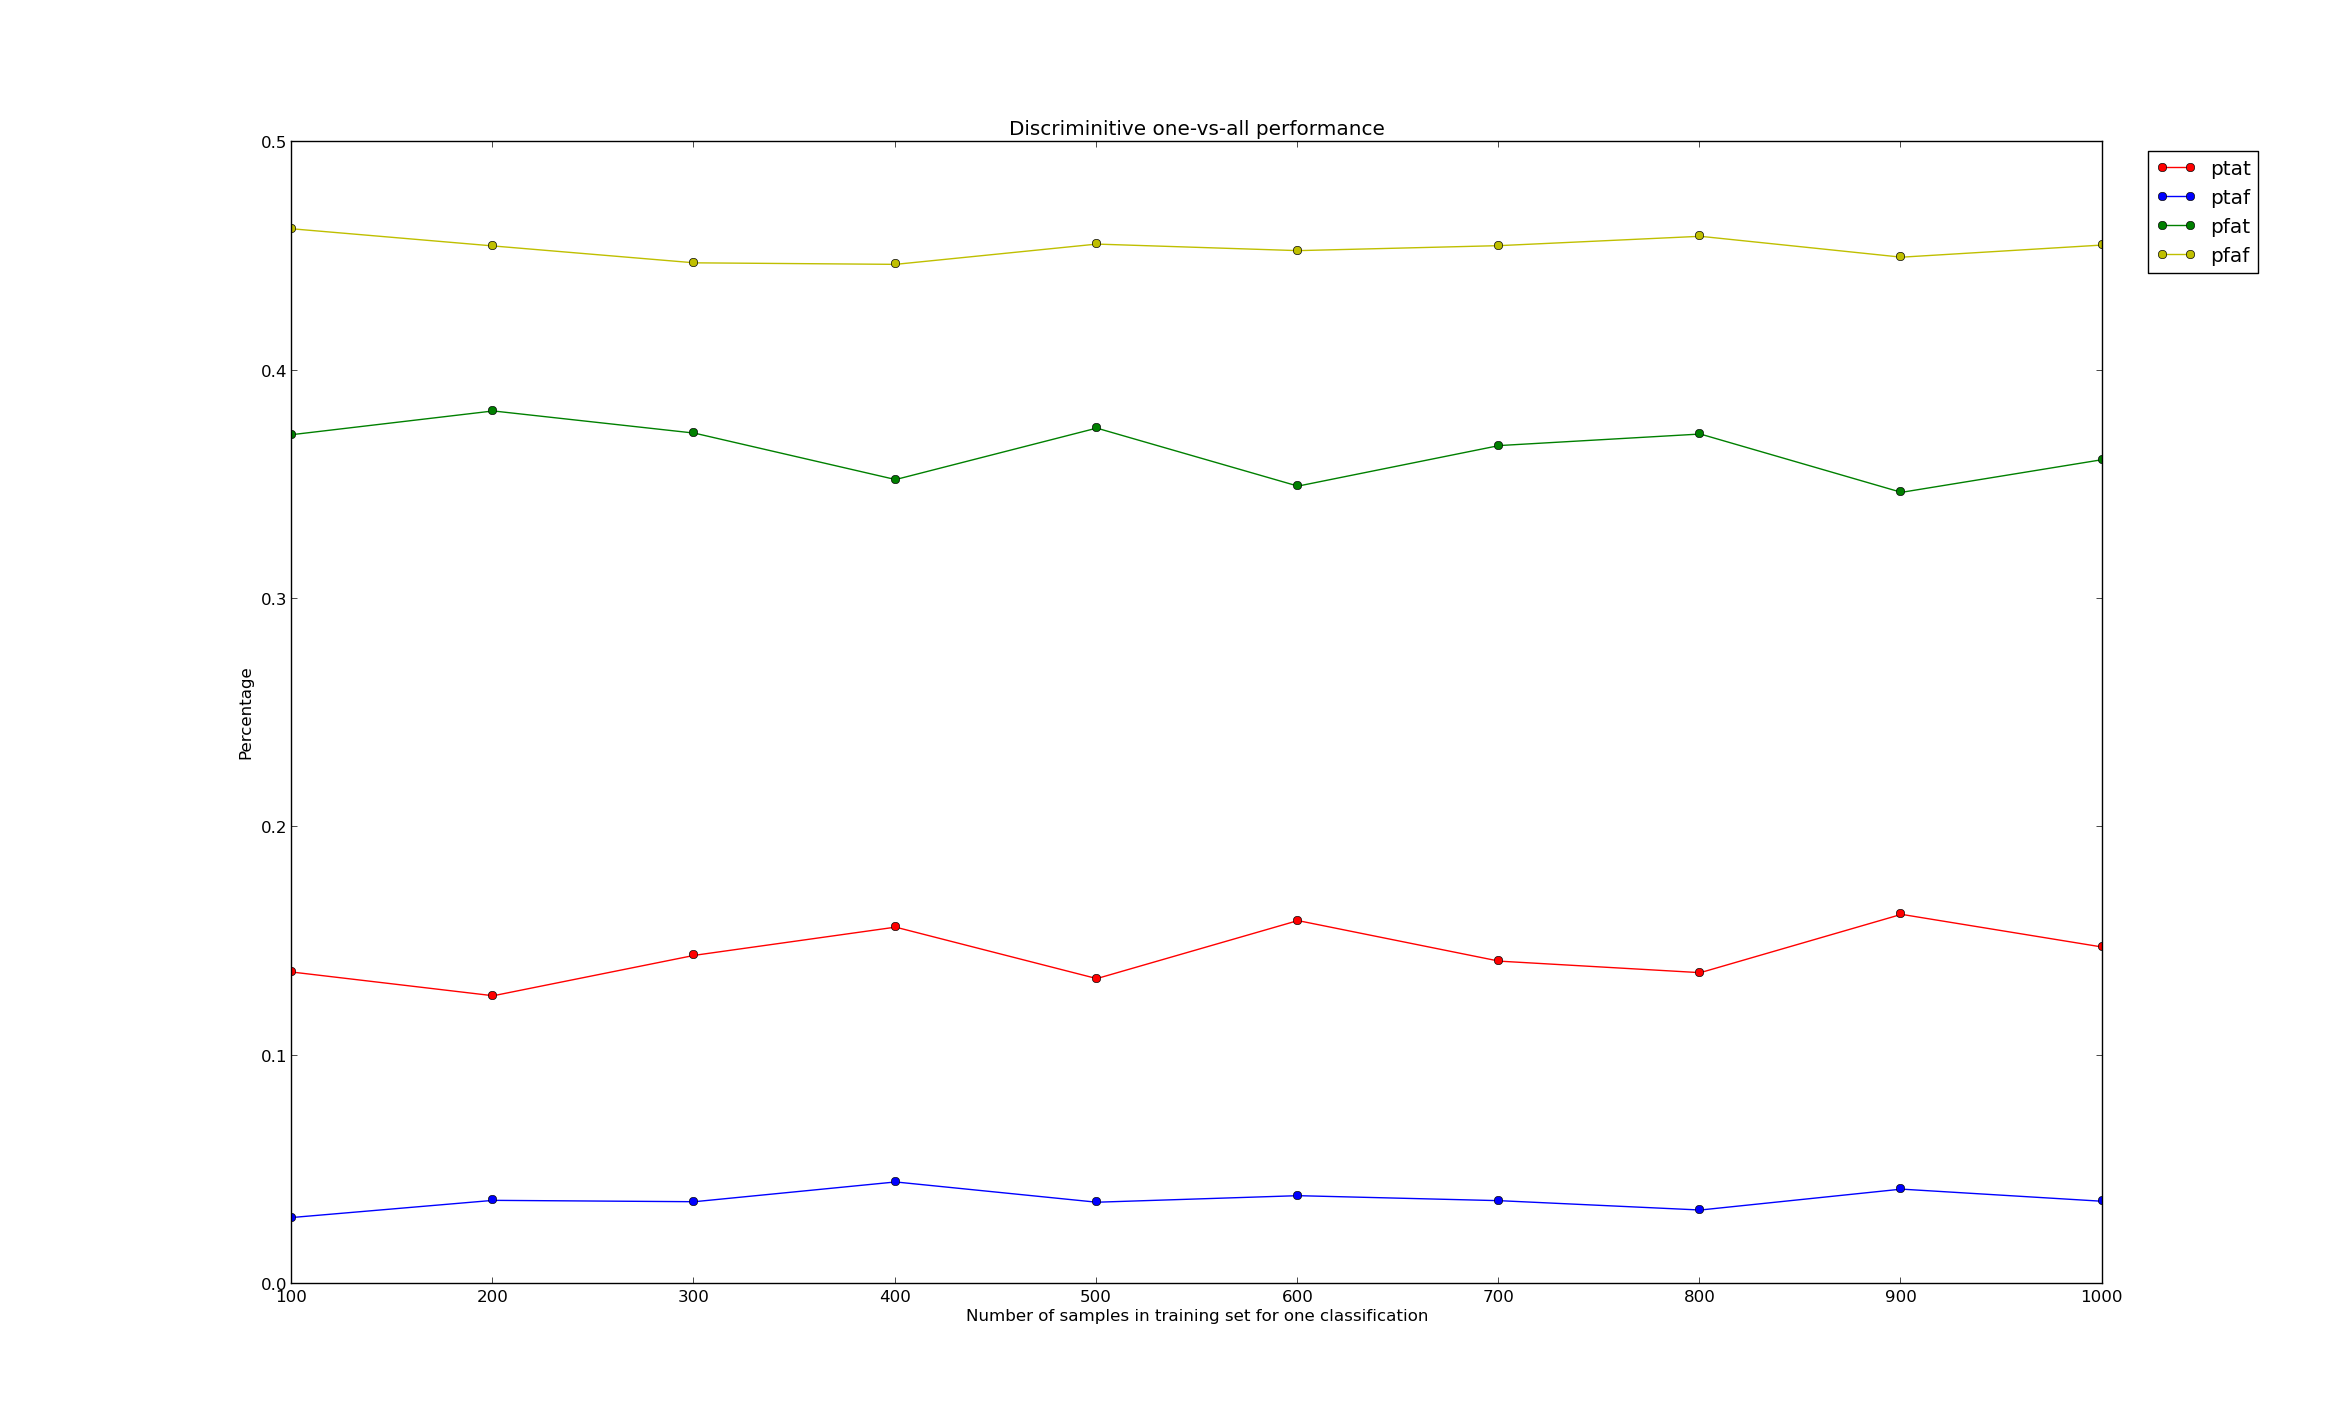
\includegraphics[scale=.15]{discriminitive.png}
\caption{Charts the ability of the classifier. Red = predicted true, actual true. Blue = predictive positive, actual negative. Green = predicted negative, actual positive. Yellow = predicted negative, actual negative.} 
\end{figure}


\section{Further Work}


\section{Conclusion}

BLAH BLAH BLAH

% In the unusual situation where you want a paper to appear in the
% references without citing it in the main text, use \nocite
%\nocite{langley00}




\section{Introductory Figures}
\begin{figure}
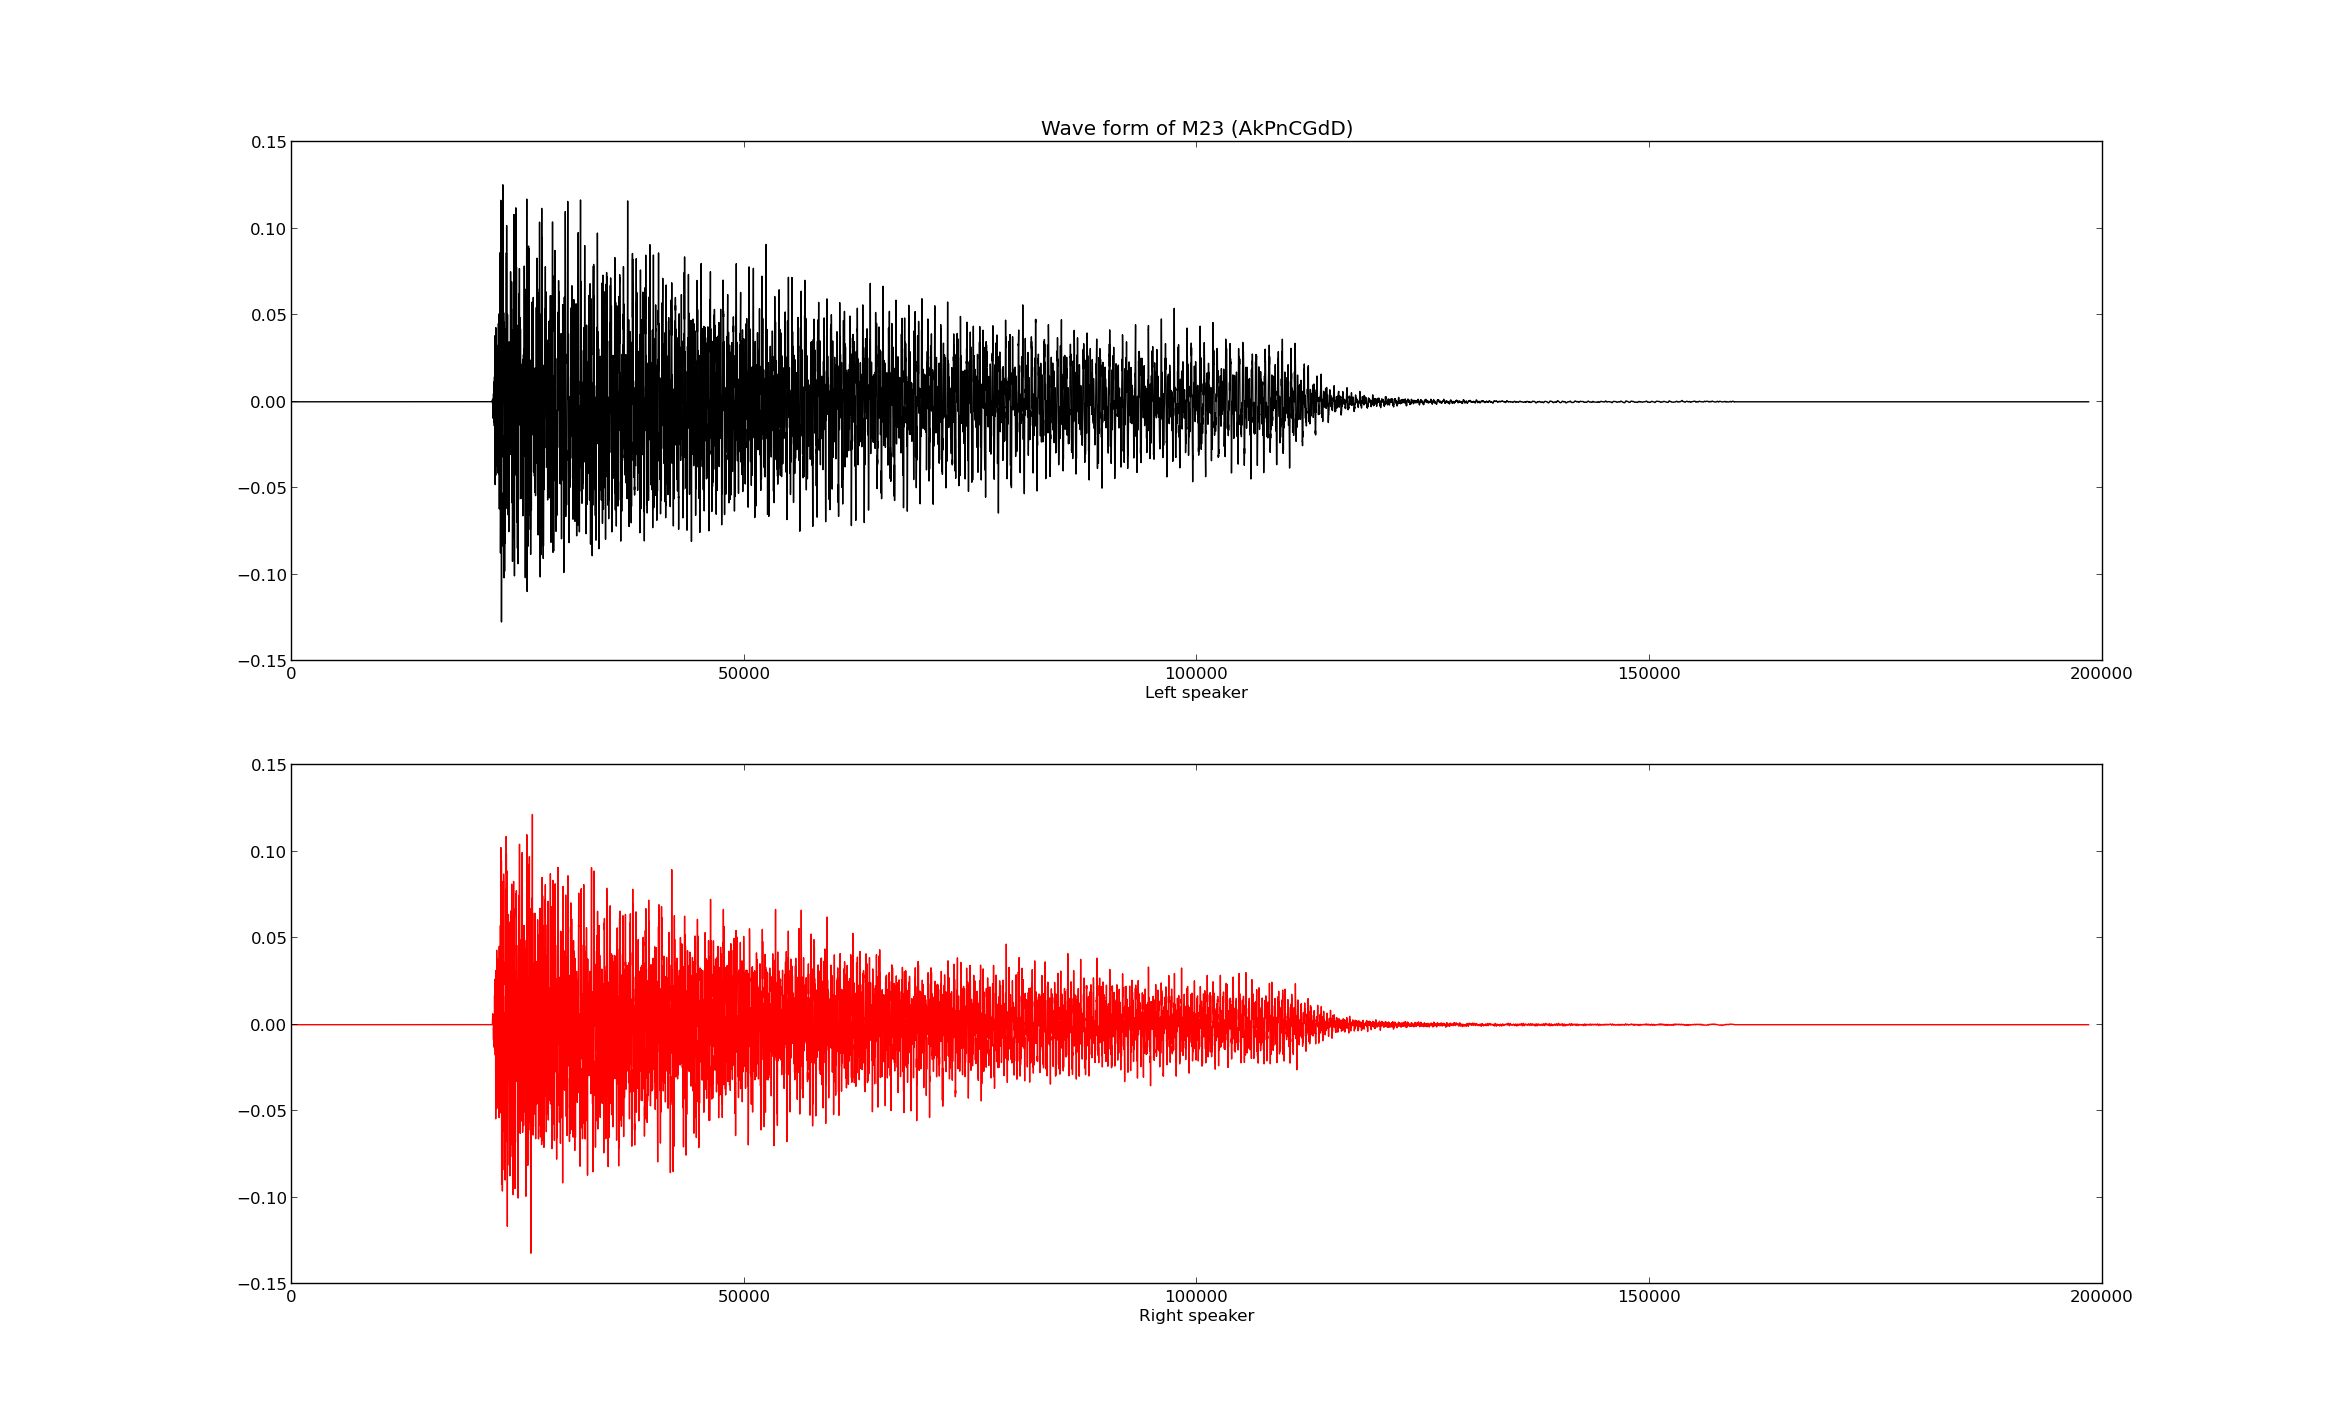
\includegraphics[scale=.13]{wave_m23.png}
\caption{Wave of C1 (Low C)}
\label{fig:wave}
\end{figure}

\begin{figure}
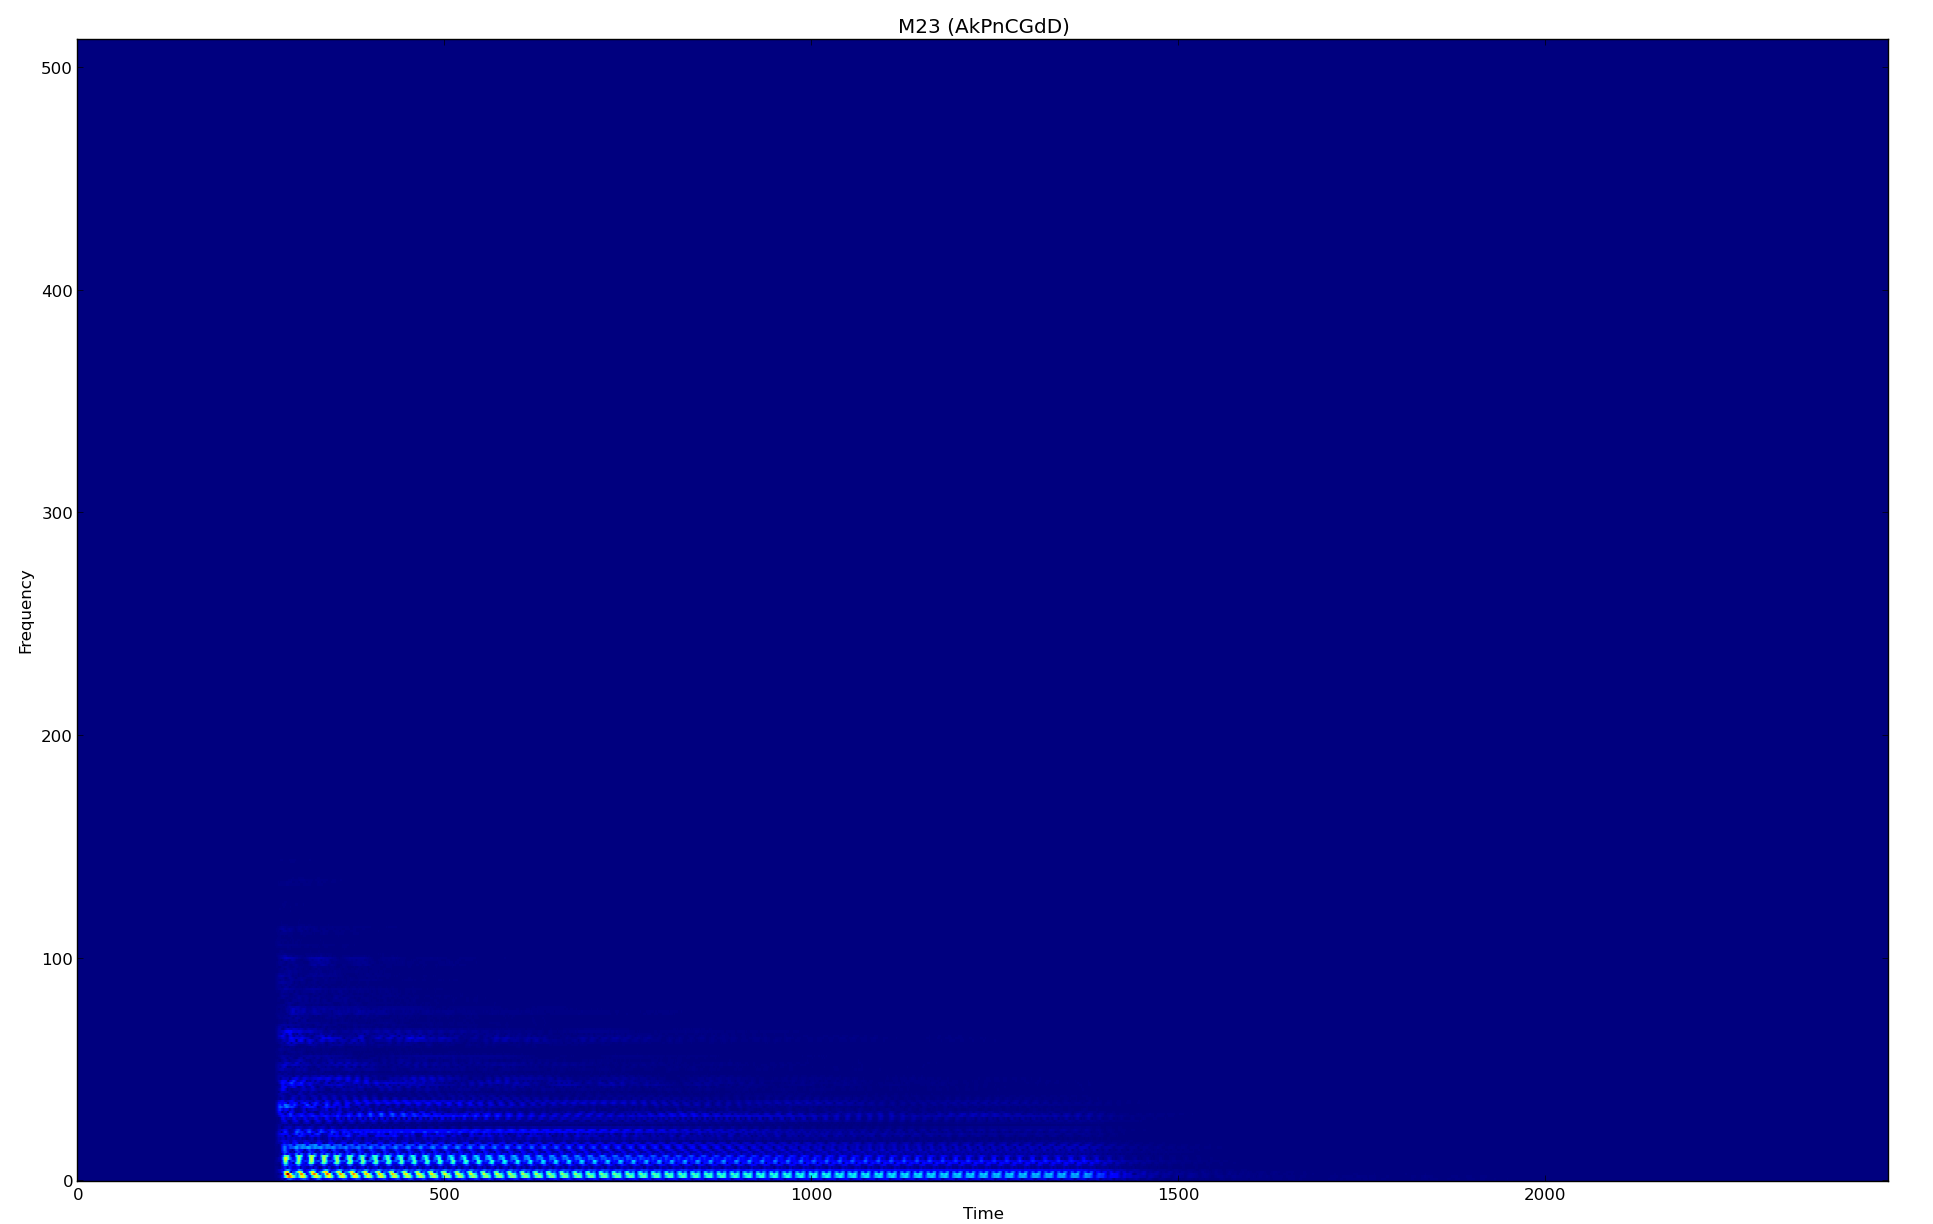
\includegraphics[scale=.12]{freq_m23.png}
\caption{Frequency map of note C1 (Low C)}
\label{fig:freqs}
\end{figure}

\begin{figure}
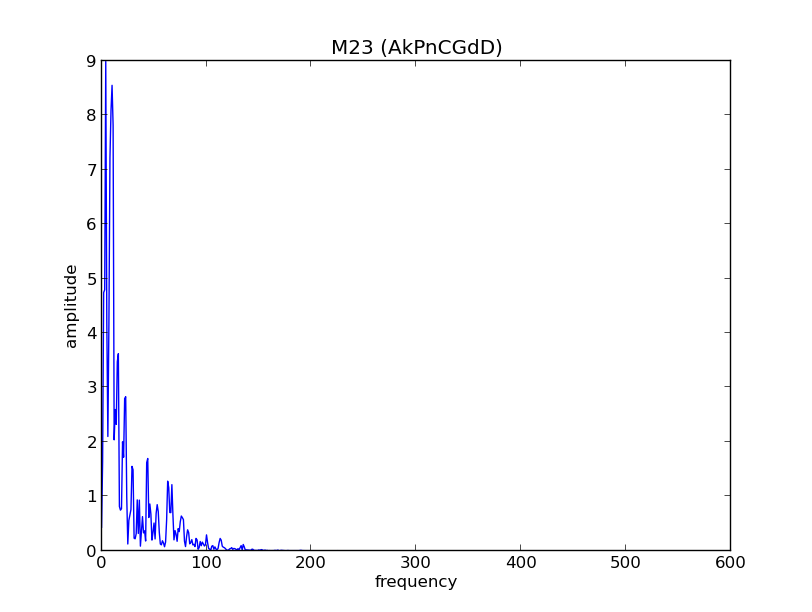
\includegraphics[scale=.4]{singlefreq_m23.png}
\caption{Frequency graph shortly after onset of C1 (Low C)}
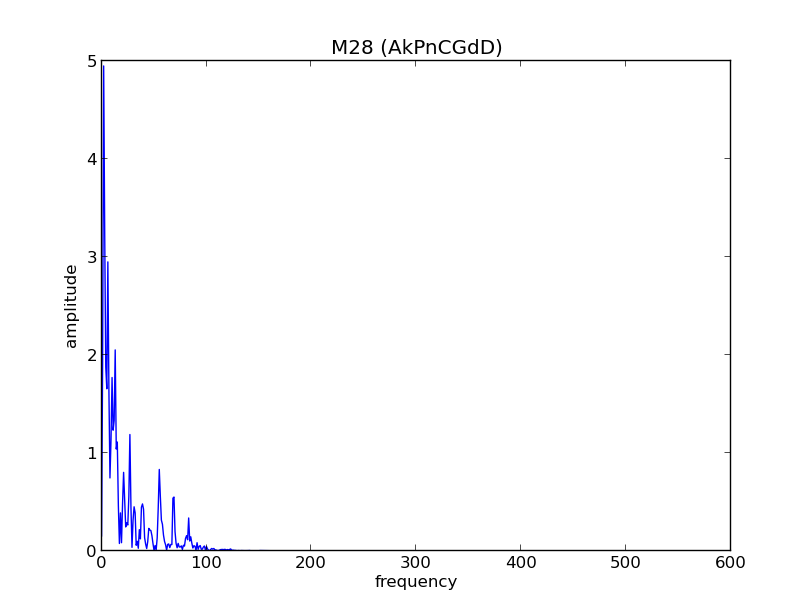
\includegraphics[scale=.4]{singlefreq_m28.png}
\caption{Frequency graph shortly after onset of E1 (Low E)}
\label{fig:single_freqs}
\end{figure}

\bibliography{finalreport}
\bibliographystyle{icml2010}

\end{document} 


% This document was modified from the file originally made available by
% Pat Langley and Andrea Danyluk for ICML-2K. This 2010 version was
% created by Thorsten Joachims & Johannes Fuernkranz, 
% slightly modified from the 2009 version by Kiri Wagstaff and 
% Sam Roweis's 2008 version, which is slightly modified from 
% Prasad Tadepalli's 2007 version which is a lightly 
% changed version of the previous year's version by Andrew Moore, 
% which was in turn edited from those of Kristian Kersting and 
% Codrina Lauth. Alex Smola contributed to the algorithmic style files.  


